\section*{Appendix A - Harricana River dataset}

\renewcommand{\arraystretch}{1.2}
\begin{table}[H]
\centering
\caption{Flow measurements (CMS) by year for the Harricana River dataset.}
\begin{tabular}{l c | l c | l c}
\hline
\textbf{Year} & \textbf{Flow} & \textbf{Year} & \textbf{Flow} & \textbf{Year} & \textbf{Flow} \\ \hline
1915 & 122   & 1938 & 240   & 1961 & 125   \\
1916 & 244   & 1939 & 230   & 1962 & 166   \\
1917 & 214   & 1940 & 192   & 1963 & 99  \\
1918 & 173   & 1941 & 195   & 1964 & 202   \\
1919 & 229   & 1942 & 172   & 1965 & 230   \\
1920 & 156   & 1943 & 173   & 1966 & 158   \\
1921 & 212   & 1944 & 172   & 1967 & 262   \\
1922 & 263   & 1945 & 153   & 1968 & 154   \\
1923 & 146   & 1946 & 142   & 1969 & 164   \\
1924 & 183   & 1947 & 317   & 1970 & 182   \\
1925 & 161   & 1948 & 161   & 1971 & 164   \\
1926 & 205   & 1949 & 201   & 1972 & 183   \\
1927 & 135   & 1950 & 204   & 1973 & 171   \\
1928 & 331   & 1951 & 194   & 1974 & 250   \\
1929 & 225   & 1952 & 164   & 1975 & 184   \\
1930 & 174   & 1953 & 183   & 1976 & 205   \\
1931 & 99  & 1954 & 161   & 1977 & 237   \\
1932 & 149   & 1955 & 167   & 1978 & 177   \\
1933 & 238   & 1956 & 179   & 1979 & 239   \\
1934 & 262   & 1957 & 185   & 1980 & 187   \\
1935 & 132   & 1958 & 117   & 1981 & 180   \\
1936 & 235   & 1959 & 192   & 1982 & 173   \\
1937 & 216   & 1960 & 337   & 1983 & 174   \\ \hline
\end{tabular}
\label{table:HRA_flows}
\end{table}


\section*{Appendix B - Fisher Dam dataset}

\renewcommand{\arraystretch}{1.2}
\begin{table}[H]
\centering
\caption{Flow measurements (CMS) by year for the Fisher Dam dataset (rounded to integers).}
\begin{tabular}{l c | l c | l c}
\hline
\textbf{Year} & \textbf{Flow} & \textbf{Year} & \textbf{Flow} & \textbf{Year} & \textbf{Flow} \\ \hline
1916 & 14   & 1943 & 6    & 1970 & 1    \\
1917 & 35   & 1944 & 15   & 1971 & 28   \\
1918 & 110  & 1945 & 366  & 1972 & 12   \\
1919 & 148  & 1946 & 5    & 1973 & 19   \\
1920 & 17   & 1947 & 138  & 1974 & 178  \\
1921 & 3    & 1948 & 473  & 1975 & 31   \\
1922 & 357  & 1949 & 134  & 1976 & 2    \\
1923 & 11   & 1950 & 44   & 1977 & 9    \\
1924 & 64   & 1951 & 23   & 1978 & 33   \\
1925 & 388  & 1952 & 6    & 1979 & 3    \\
1926 & 122  & 1953 & 137  & 1980 & 86   \\
1927 & 32   & 1954 & 55   & 1981 & 22   \\
1928 & 139  & 1955 & 13   & 1982 & 12   \\
1929 & 54   & 1956 & 35   & 1983 & 15   \\
1930 & 169  & 1957 & 632  & 1984 & 4    \\
1931 & 11   & 1958 & 10   & 1985 & 8    \\
1932 & 175  & 1959 & 84   & 1986 & 162  \\
1933 & 1    & 1960 & 8    & 1987 & 15   \\
1934 & 76   & 1961 & 99   & 1988 & 14   \\
1935 & 387  & 1962 & 6    & 1989 & 10   \\
1936 & 1149 & 1963 & 14   & 1990 & 10   \\
1937 & 117  & 1964 & 47   & 1991 & 8    \\
1938 & 93   & 1965 & 29   & 1992 & 15   \\
1939 & 5    & 1966 & 29   & 1993 & 2    \\
1940 & 27   & 1967 & 9    & 1994 & 11   \\
1941 & 73   & 1968 & 19   & 1995 & 4    \\
1942 & 10   & 1969 & 4    & 1996 & 10   \\ \hline
\end{tabular}
\label{table:OCD_flows}
\end{table}

\newpage
\section*{Appendix C - Fisher Dam: NSFFA Verification Results}

\begin{figure}[H]
    \centering
    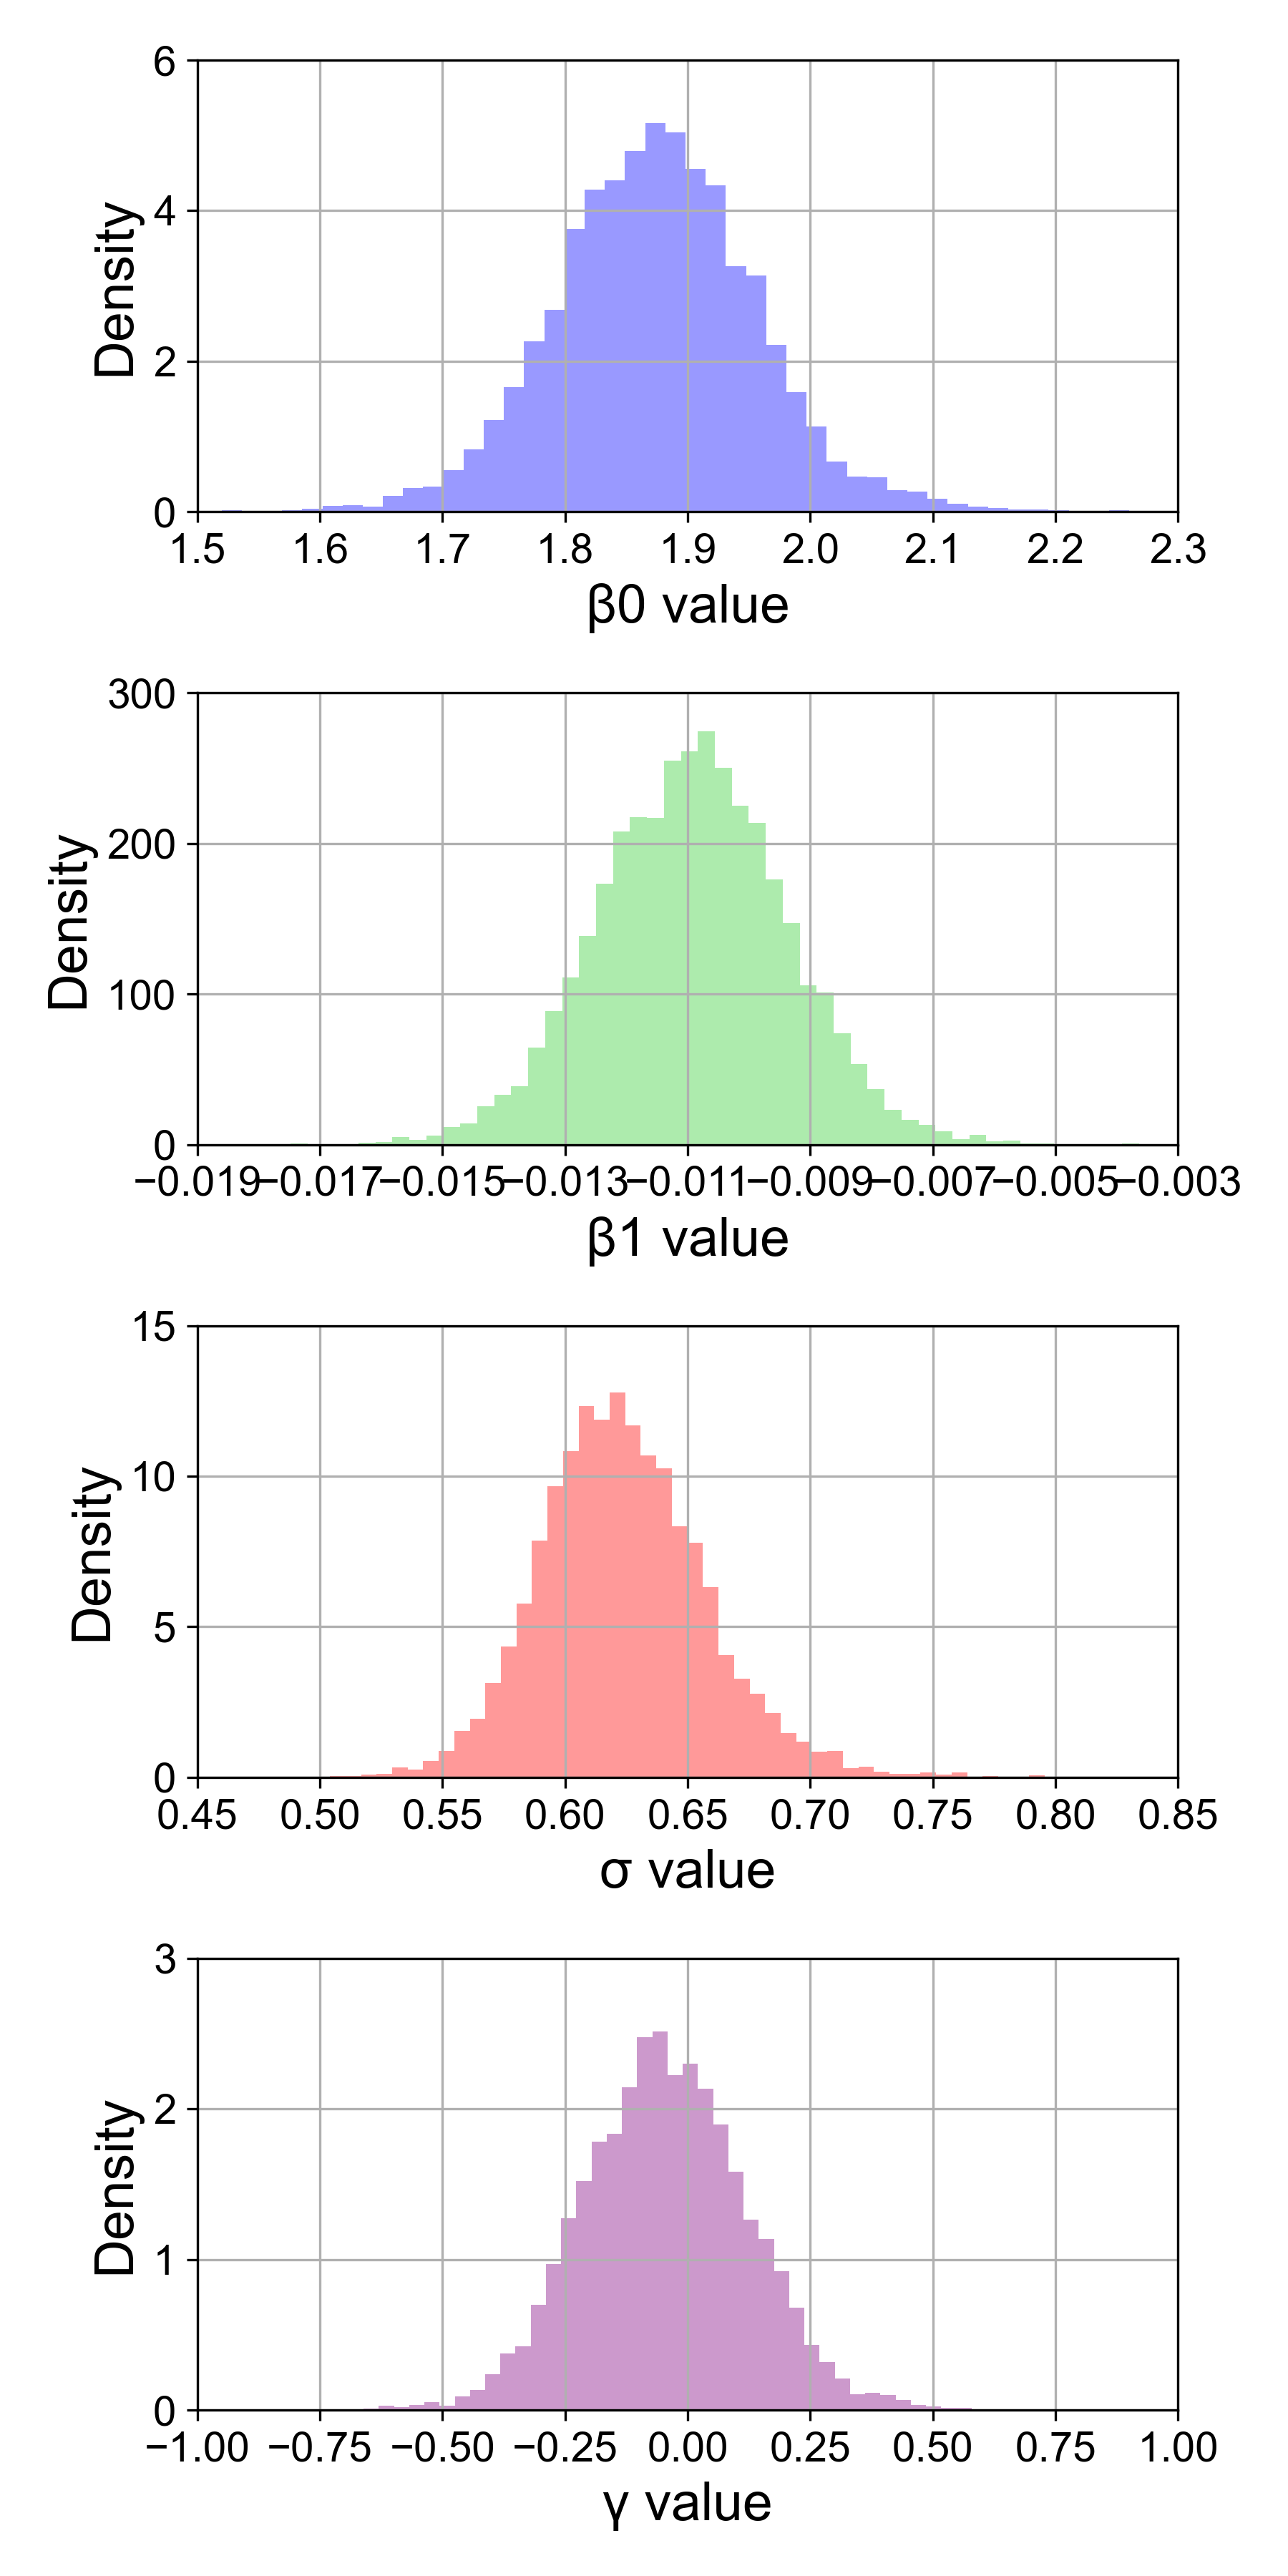
\includegraphics[width=1\linewidth]{_plots/OCD_linear_mu_posterior_marginal_lp3.png}
    \caption{Posterior marginal distributions of LP3 distribution parameters for the NSFFA model with linear trend, derived from the Fisher Dam dataset.}
    \label{fig:OCD_linear_mu_posterior_marginal_lp3}
\end{figure}

\begin{figure}[H]
    \centering
    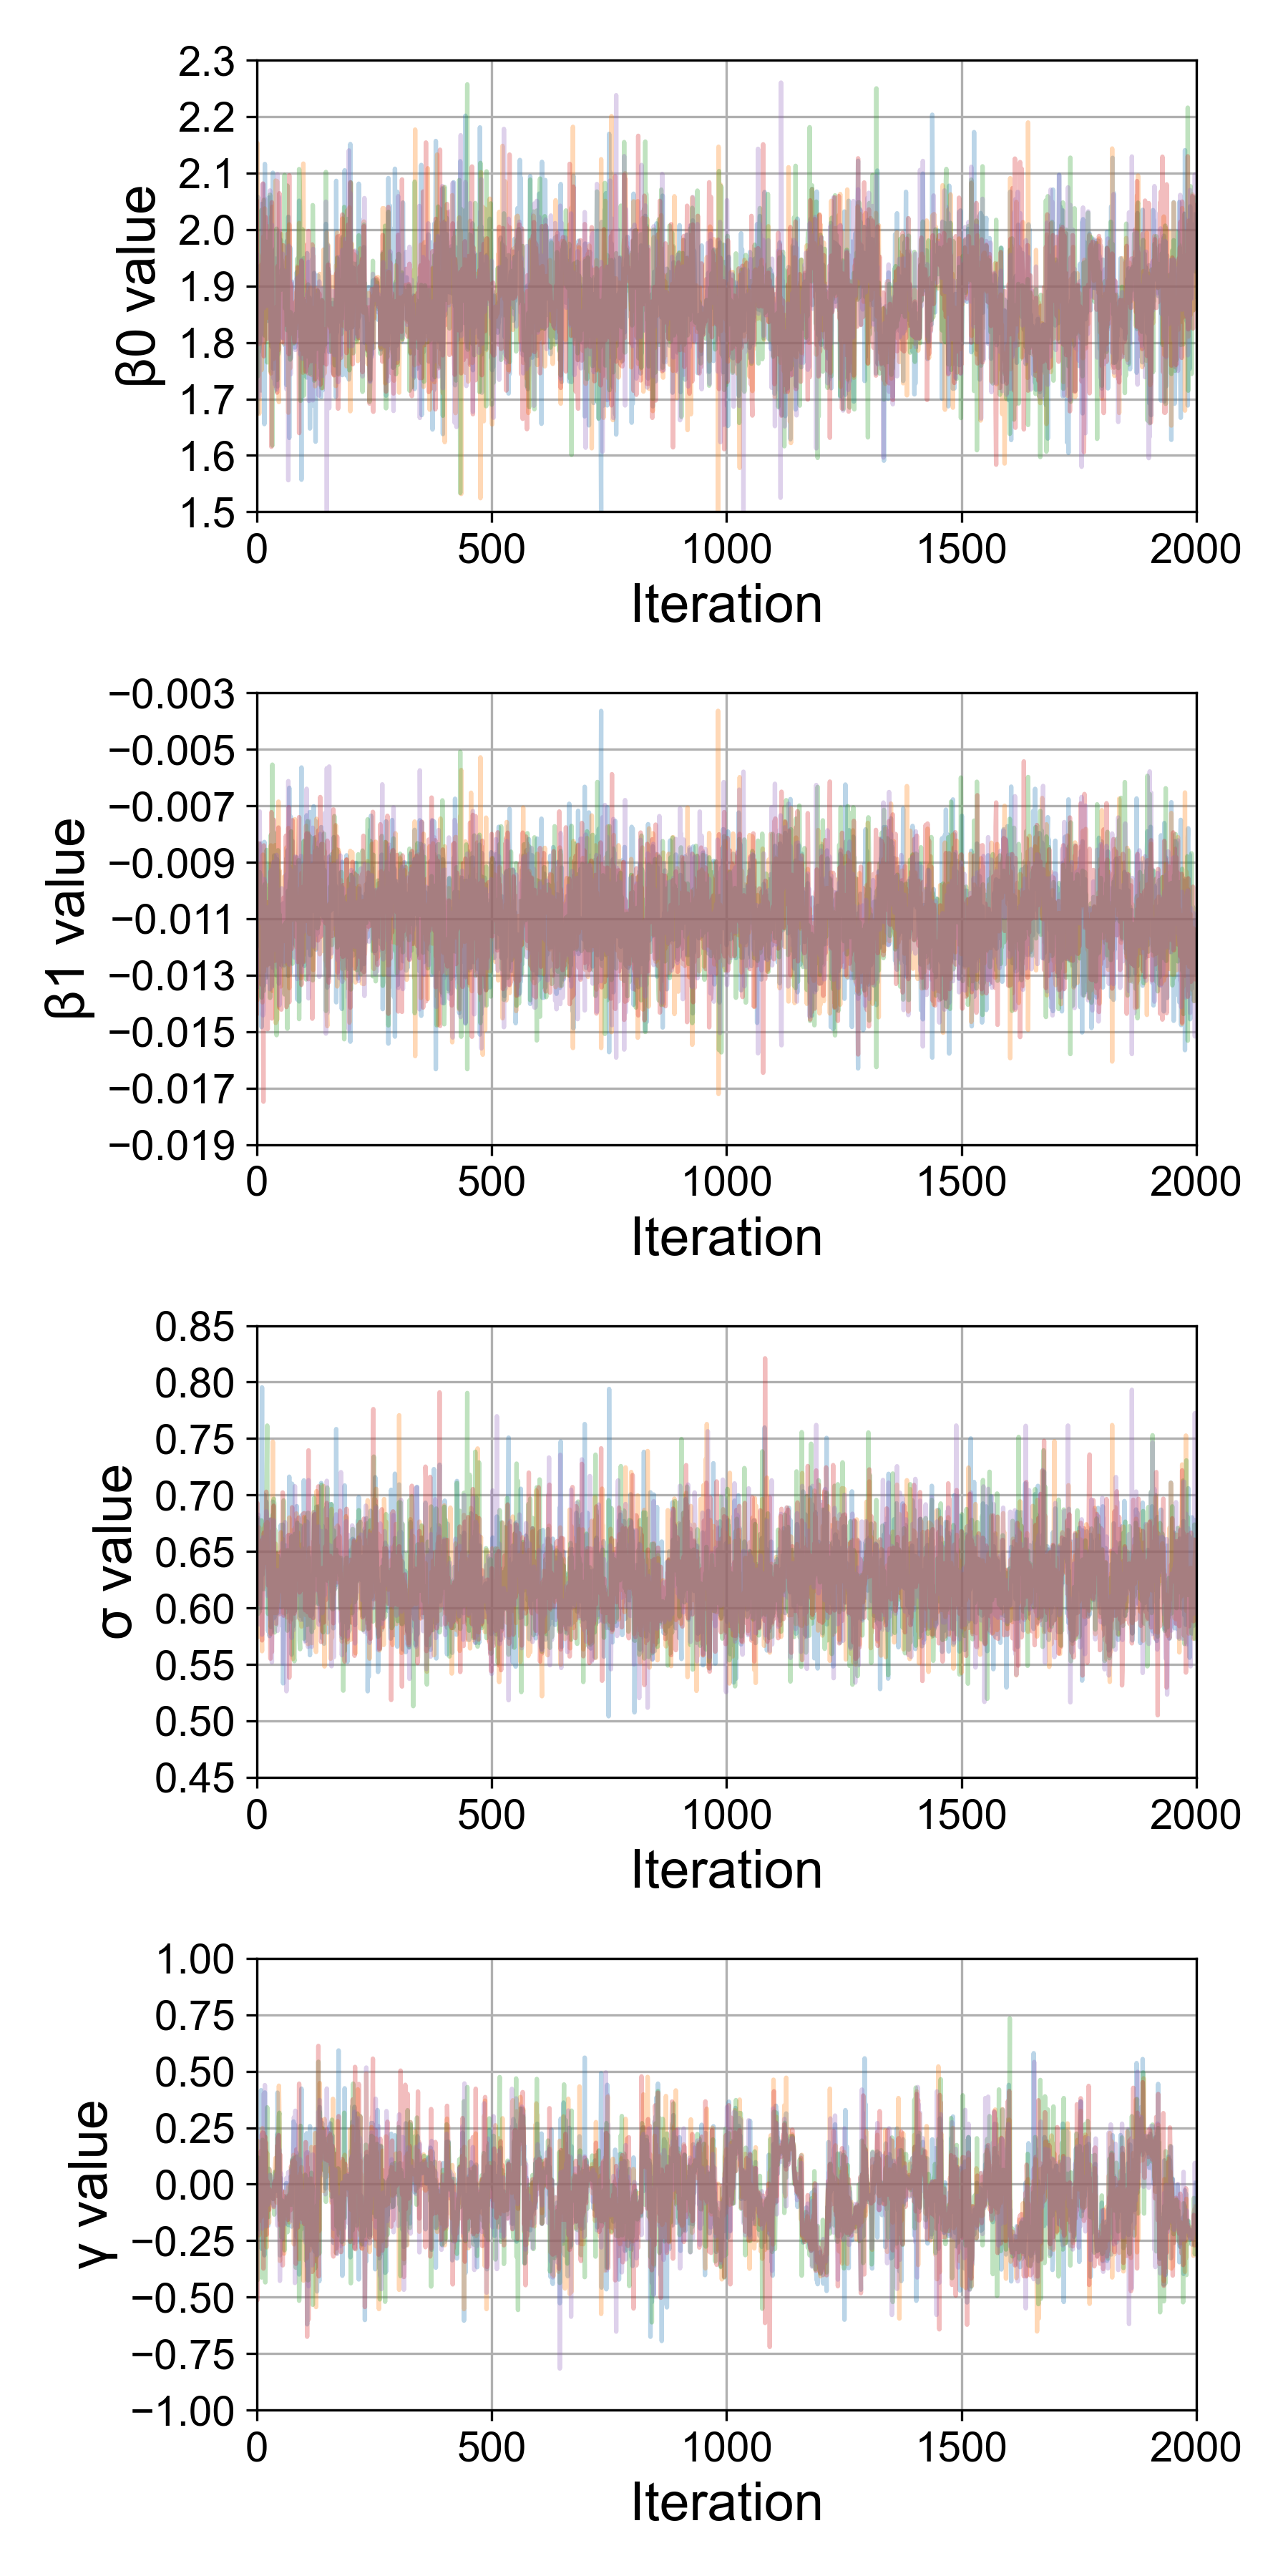
\includegraphics[width=1\linewidth]{_plots/OCD_linear_mu_posterior_trace_lp3.png}
    \caption{Trace plots of LP3 distribution parameters for the NSFFA model with linear trend, derived from the Fisher Dam dataset.}
    \label{fig:OCD_linear_mu_posterior_trace_lp3}
\end{figure}

\newpage
\begin{figure}[H]
    \centering
    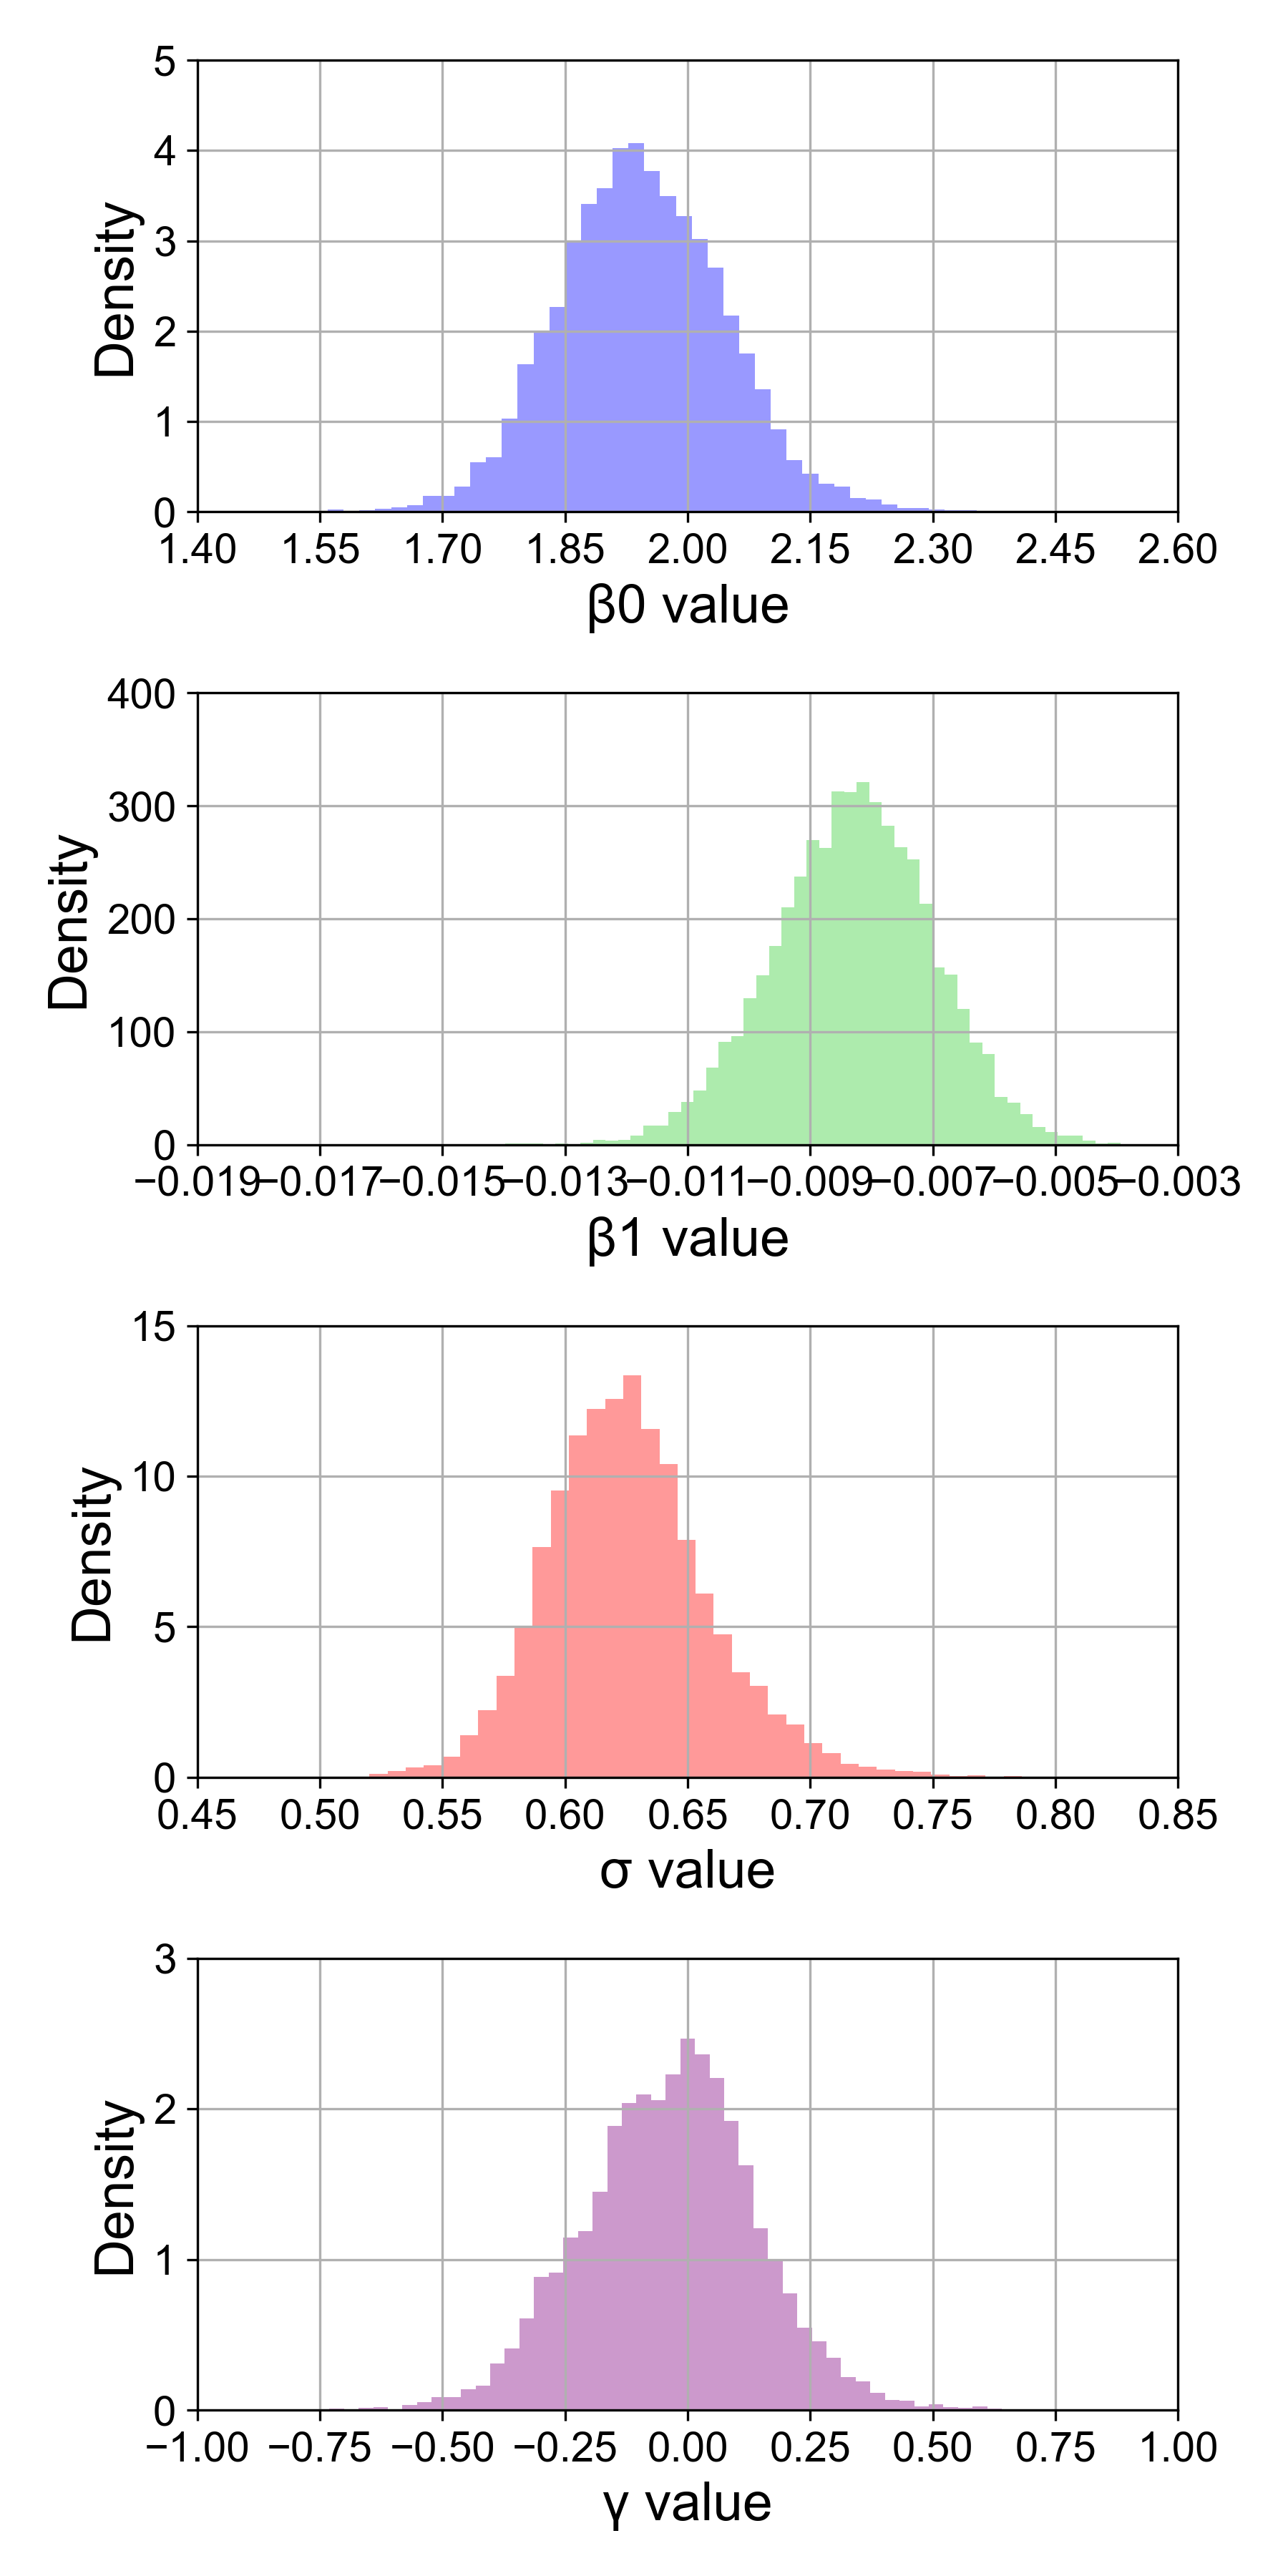
\includegraphics[width=1\linewidth]{_plots/OCD_exponential_mu_posterior_marginal_lp3.png}
    \caption{Posterior marginal distributions of LP3 distribution parameters for the NSFFA model with exponential trend, derived from the Fisher Dam dataset.}
    \label{fig:OCD_exponential_mu_posterior_marginal_lp3}
\end{figure}

\begin{figure}[H]
    \centering
    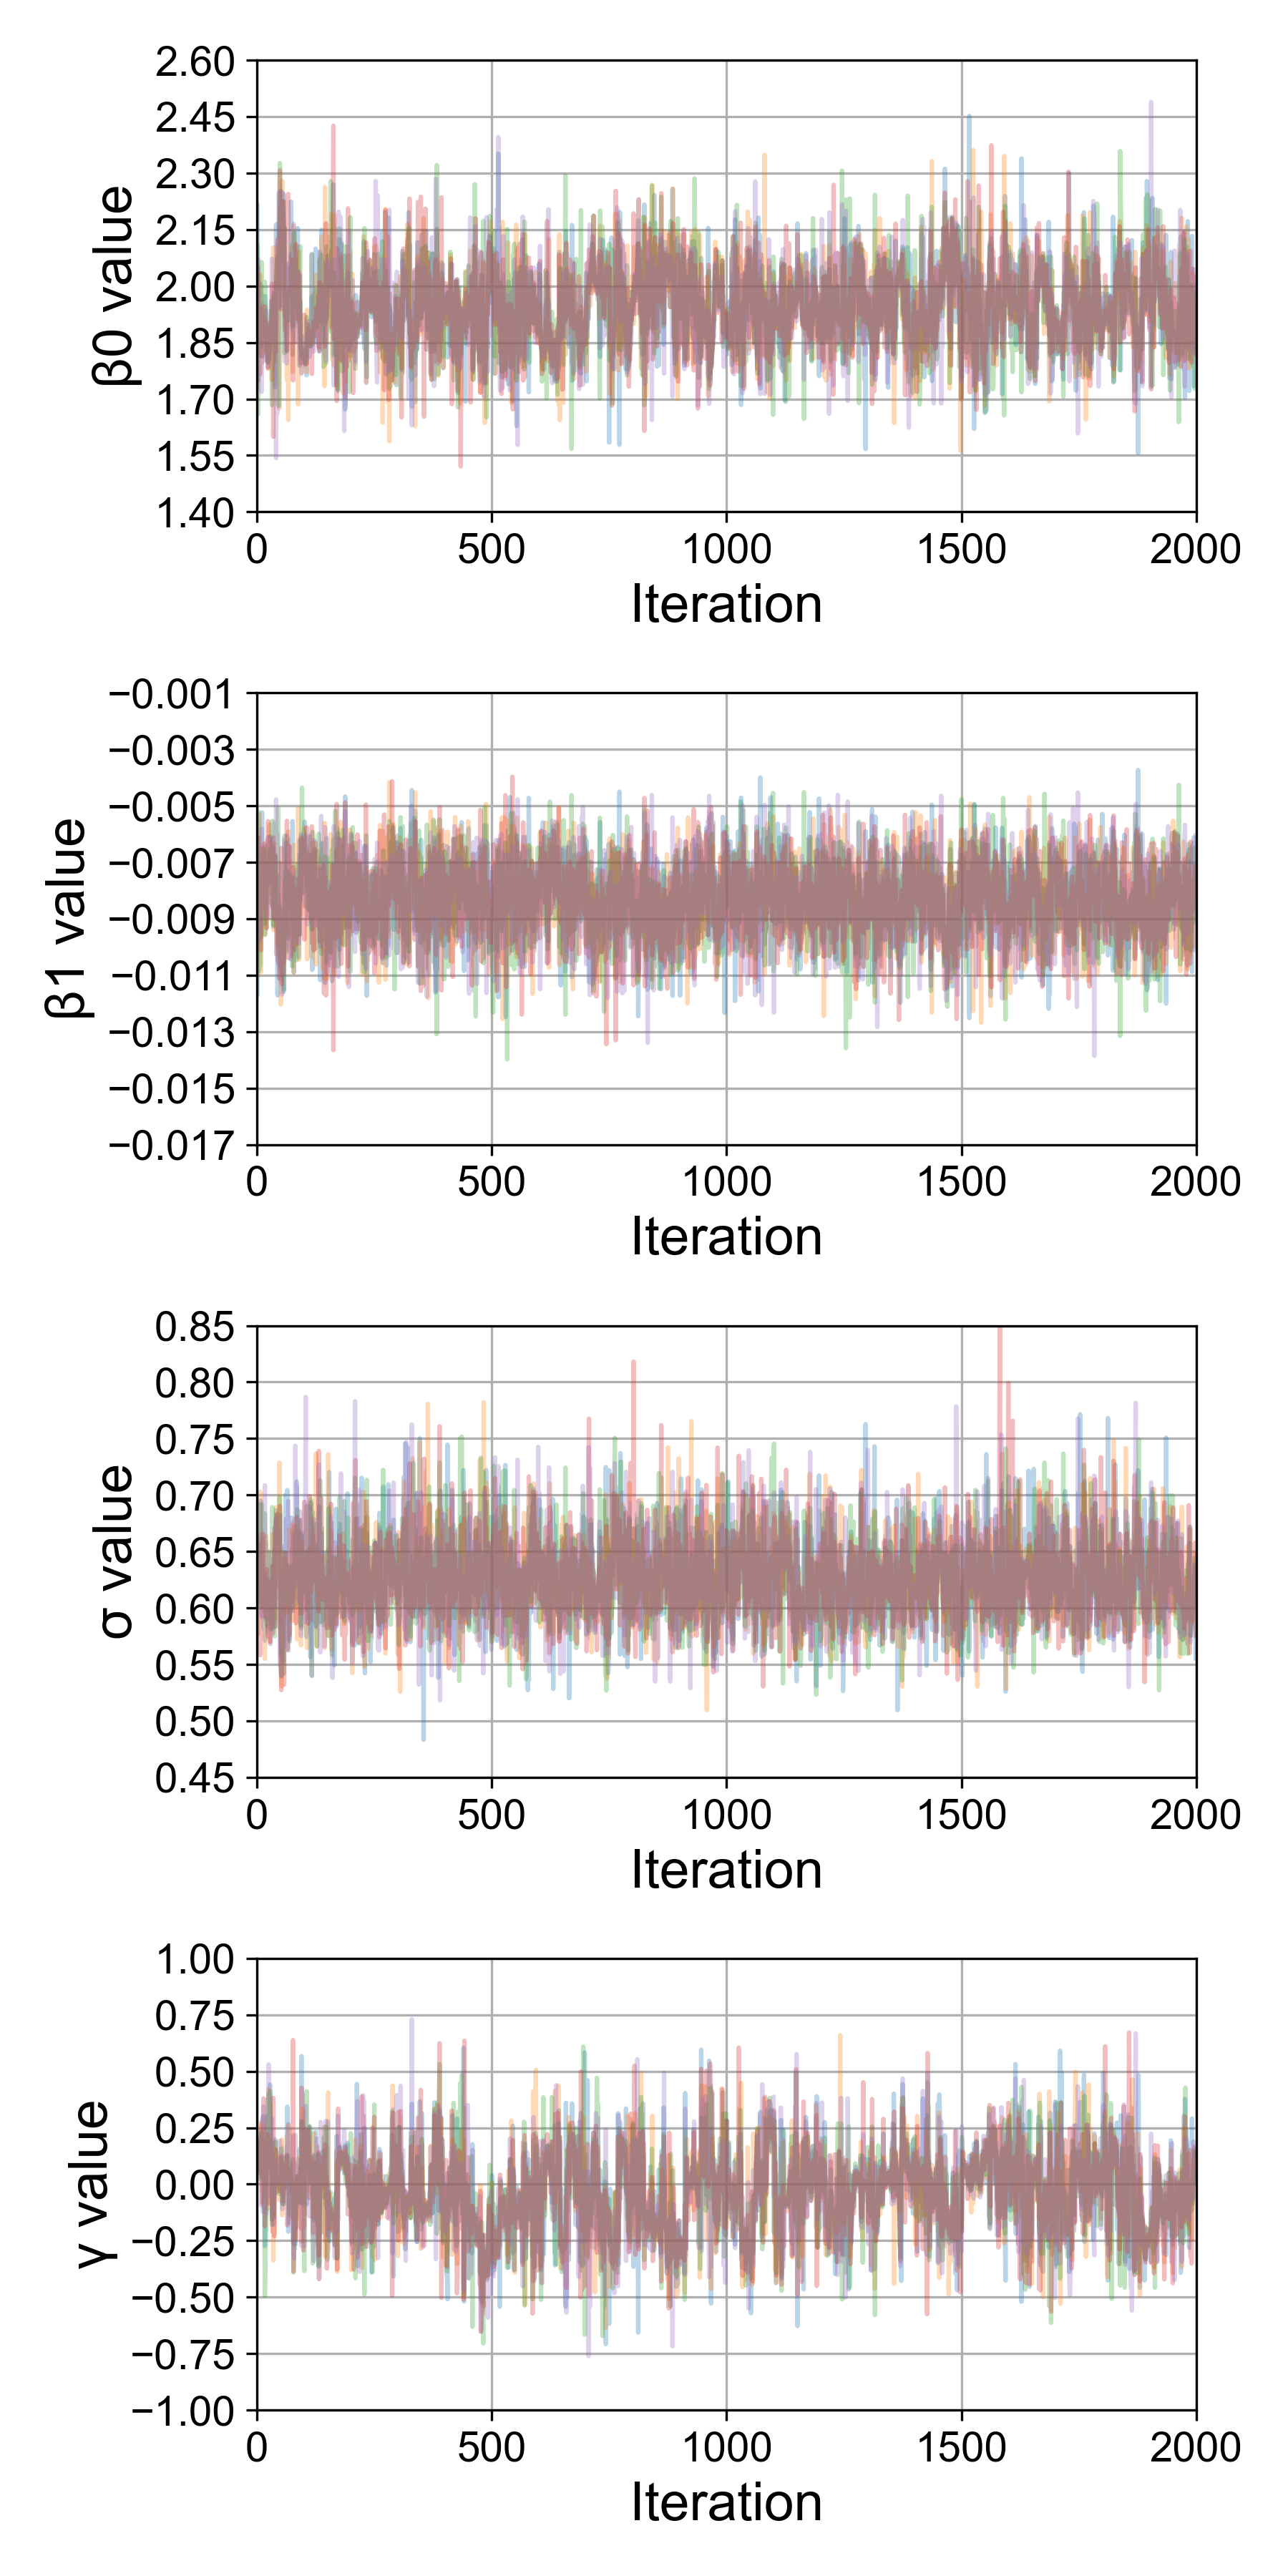
\includegraphics[width=1\linewidth]{_plots/OCD_exponential_mu_posterior_trace_lp3.png}
    \caption{Trace plots of LP3 distribution parameters for the NSFFA model with exponential trend, derived from the Fisher Dam dataset.}
    \label{fig:OCD_exponential_mu_posterior_trace_lp3}
\end{figure}

\newpage
\begin{figure*}[htp]
    \centering
    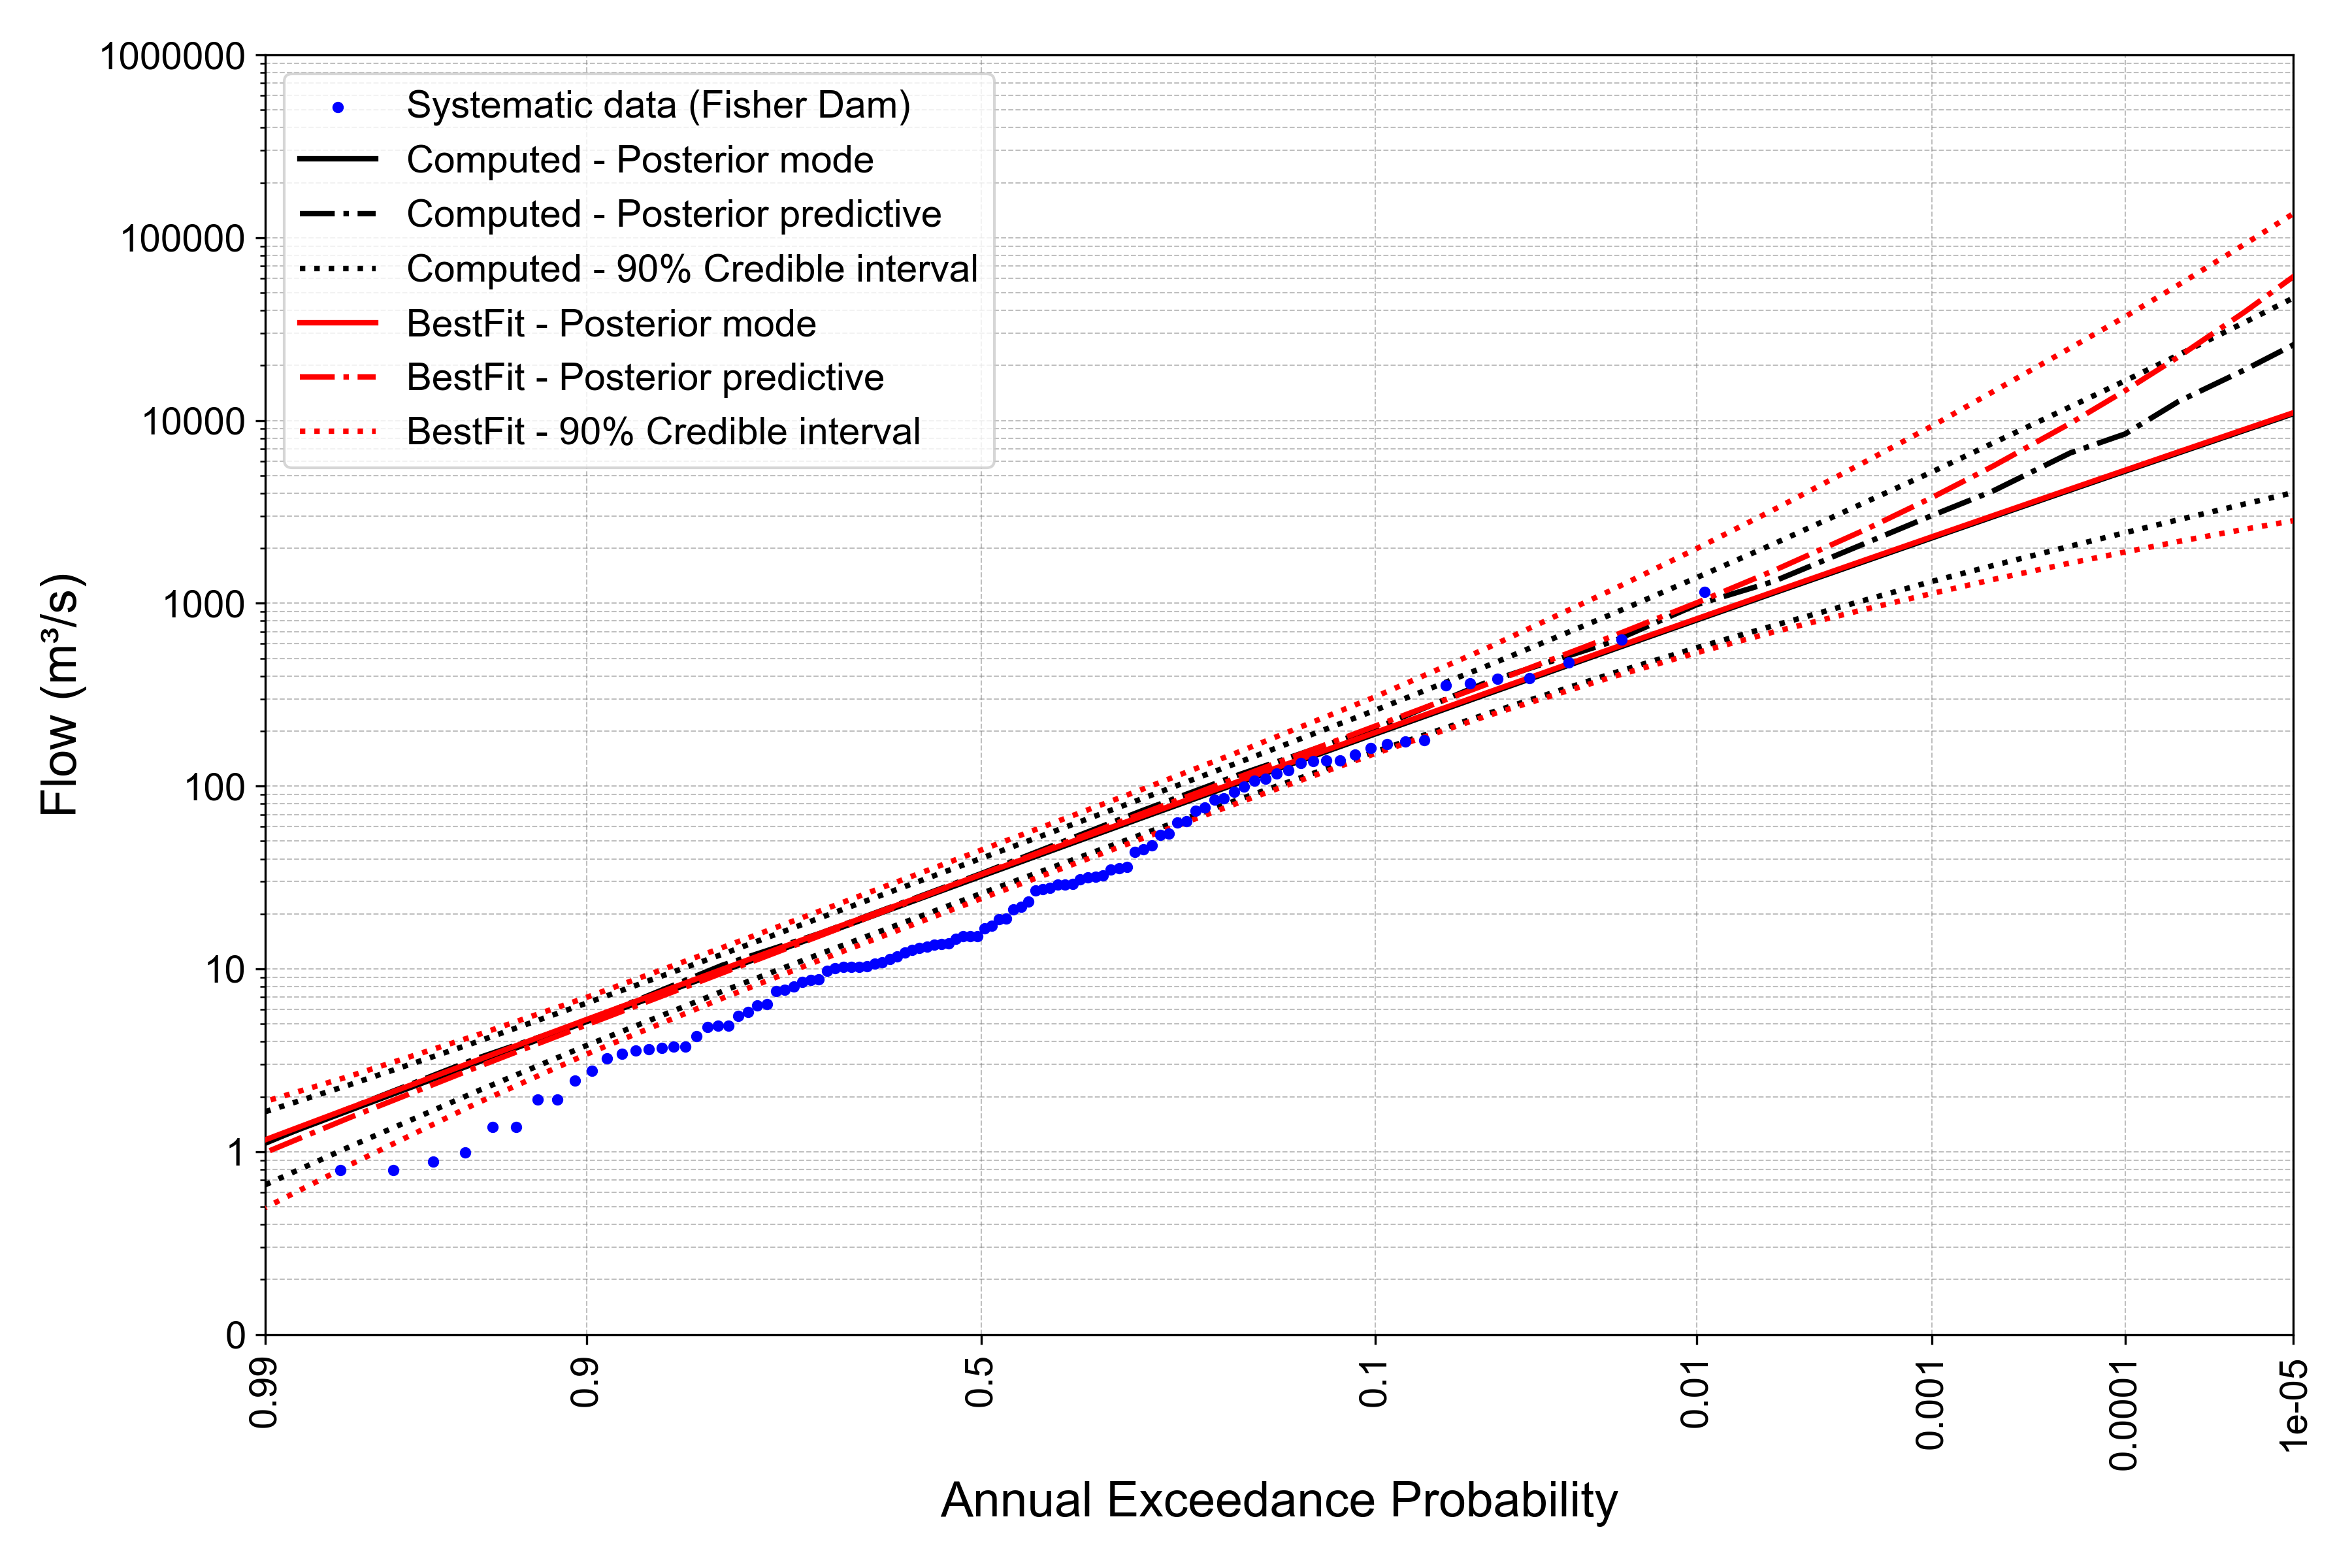
\includegraphics[width=1\linewidth]{_plots/OCD_bayesian_flood_quantiles_lp3_linear_mu.png}
    \caption{Comparison of computed Bayesian flood frequency curves with BestFit for the Fisher Dam NSFFA model with linear trend.}
    \label{fig:OCD_bayesian_flood_quantiles_lp3_linear_mu}
\end{figure*}

\begin{figure*}[htp]
    \centering
    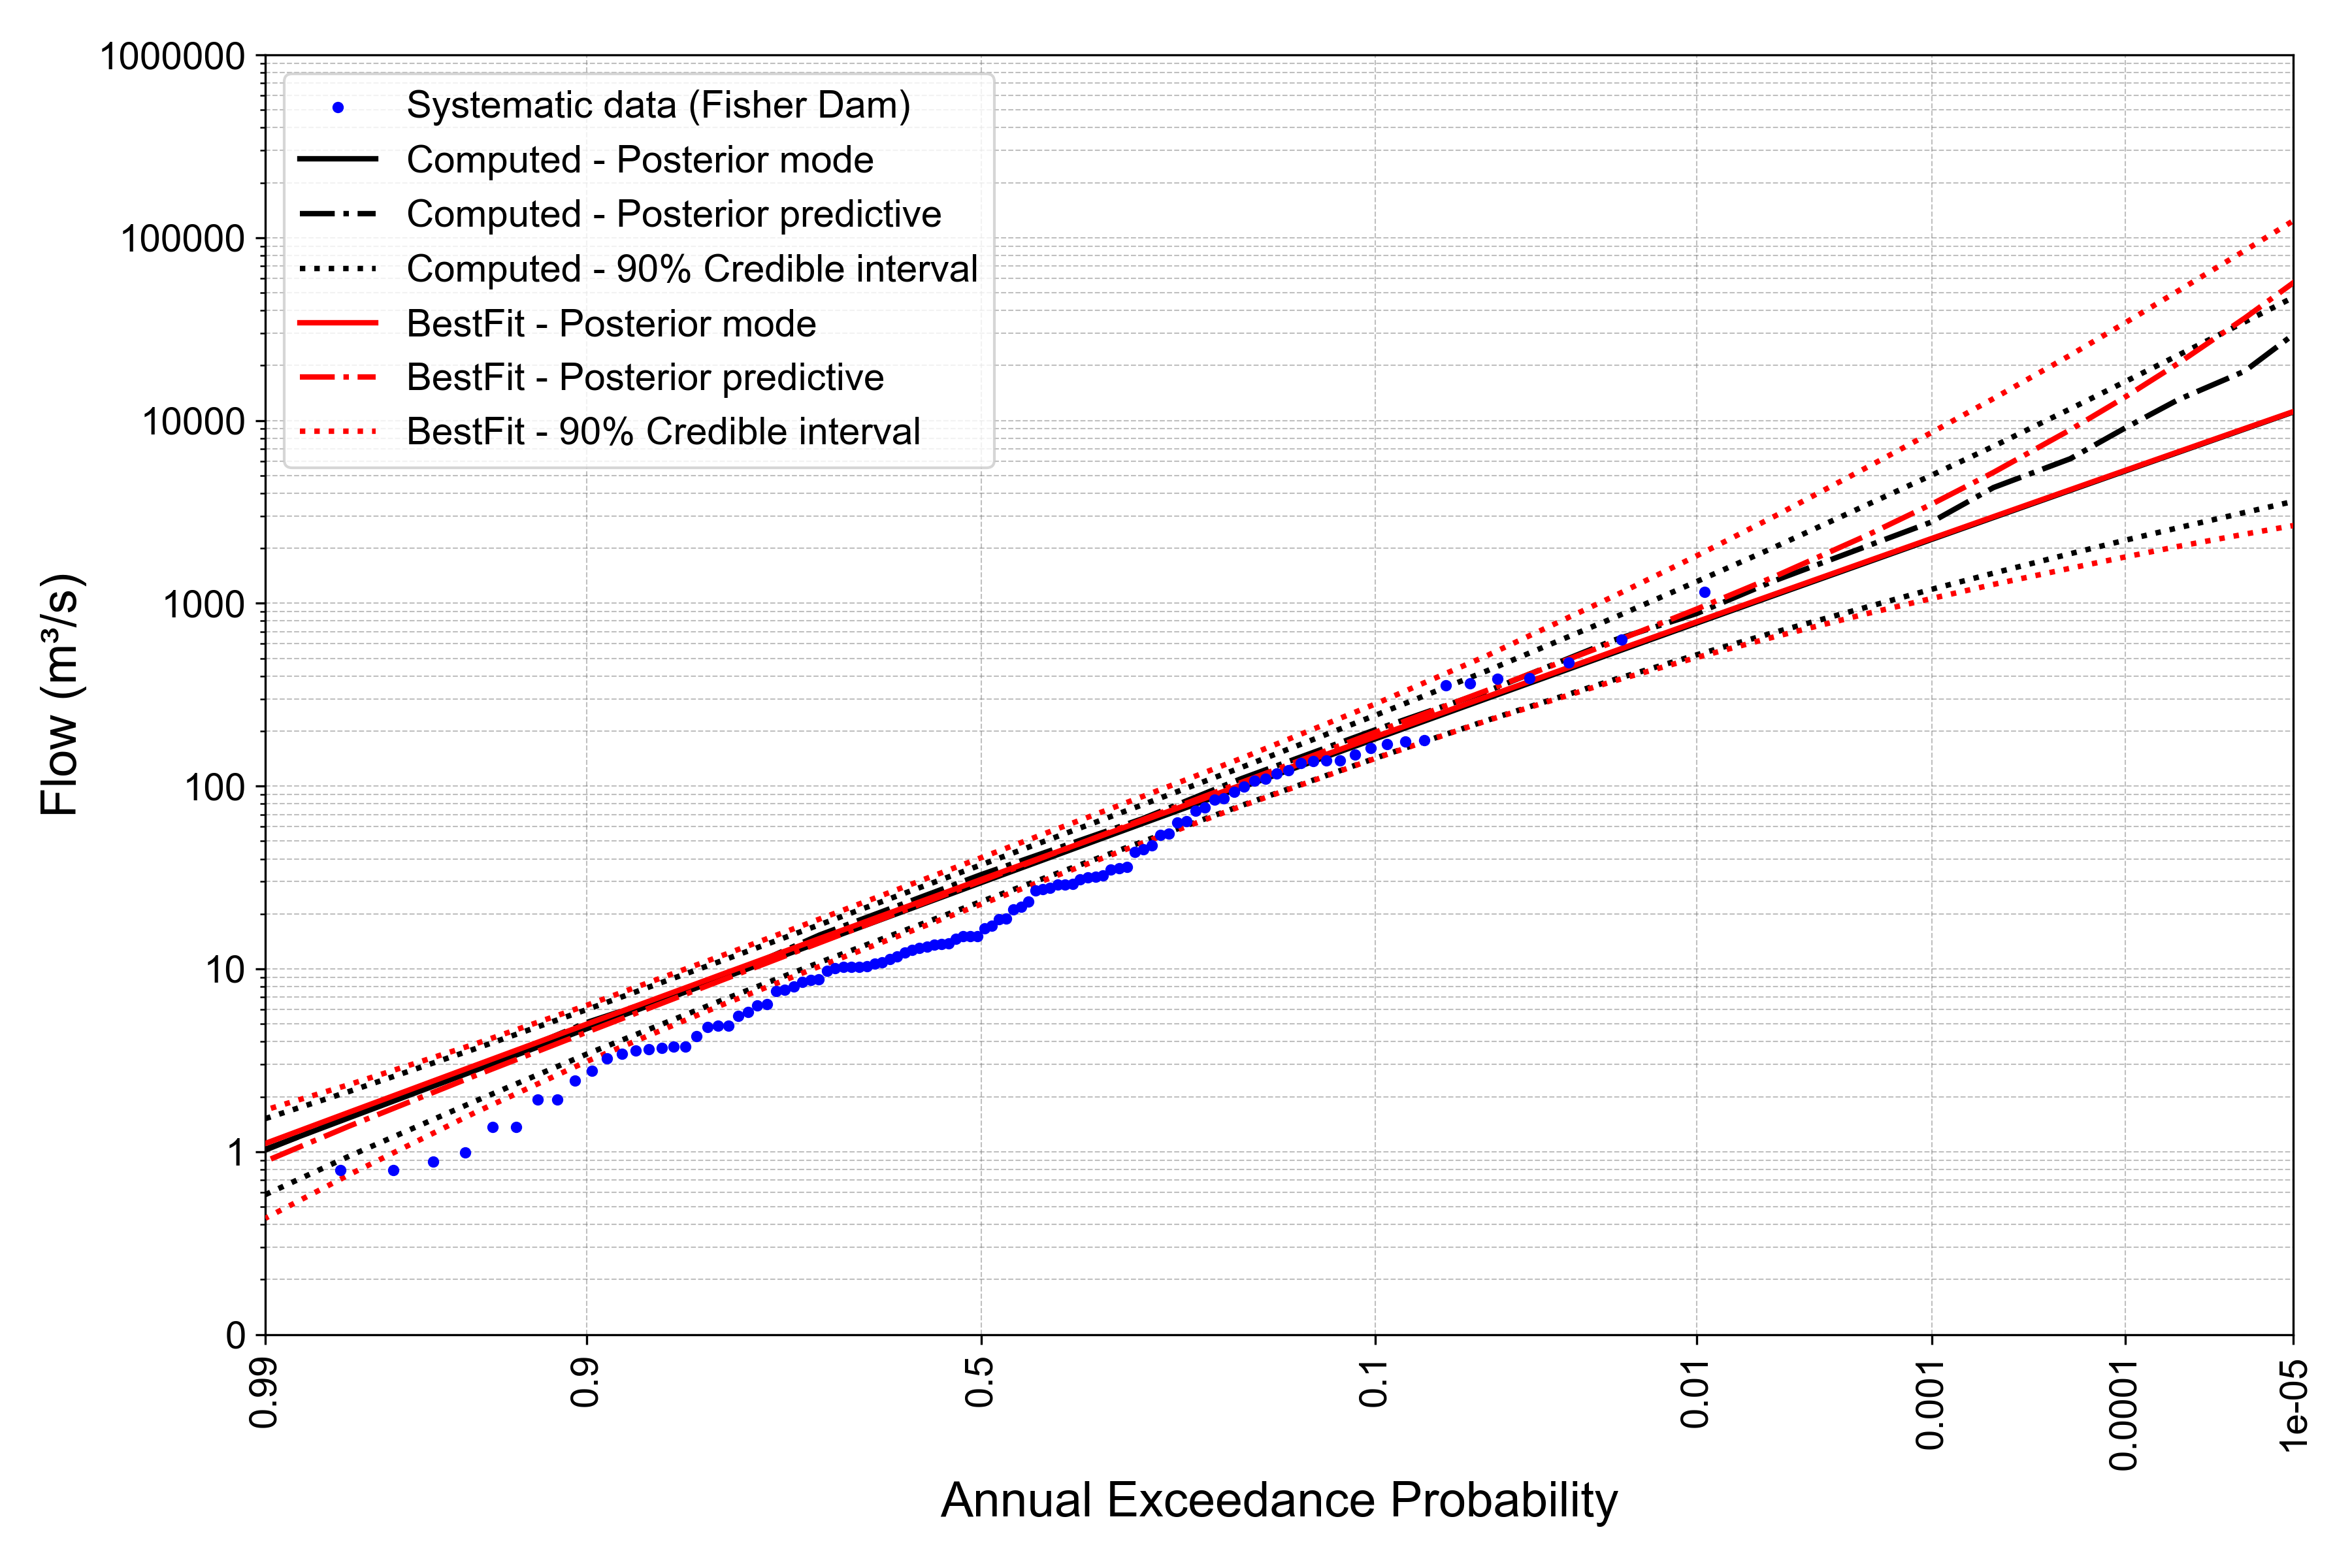
\includegraphics[width=1\linewidth]{_plots/OCD_bayesian_flood_quantiles_lp3_exponential_mu.png}
    \caption{Comparison of computed Bayesian flood frequency curves with BestFit for the Fisher Dam NSFFA model with exponential trend. }
\label{fig:OCD_bayesian_flood_quantiles_lp3_exponential_mu}
\end{figure*}

\FloatBarrier